\documentclass[pmlr,twocolumn,10pt]{jmlr}
% packages
\usepackage{booktabs}
\usepackage{graphicx}
\usepackage{subcaption}
% definitions
% (jmlr.cls in TeX Live doesn't define these JMLR-style macros; provide fallbacks.)
\providecommand{\jmlrheading}[6]{}
\providecommand{\ShortHeadings}[2]{}
\newcommand{\dataset}{{\sc Bdata}}
\newcommand{\datasetb}{{\sc Bdata}$_b$}
\begin{document}
% heading arguments: volume, year, pages (unset until publication)
\jmlrheading{1}{2026}{1-XX}{X/XX}{XX/XX}{Author et al.}
% short title for running head
\firstpageno{1}
\title{Multi-Agent Simulation of AI-Mediated Prior Authorization for Specialty Medications }
\author{\Name{Anonymous Author(s)} \Email{anonymous@anonymous.edu}\\
\addr Anonymous Institution
}
\maketitle
\begin{abstract}
Insurers and providers are both deploying AI in prior authorization, raising concerns of a prisoner's dilemma where mutual adoption produces collectively harmful outcomes. We develop a multi-agent simulation where LLM-driven provider and insurer agents negotiate authorization for a specialty medication under information asymmetry, with cooperative, adversarial, or no-guidance strategies assigned via prompts. In a 3$\times$3 factorial experiment on a single gray-zone clinical case, we find that the insurer's choice between requesting additional information and outright denial at initial review is the mechanism through which gray-zone ambiguity is resolved. Default (no-guidance) insurer agents denied the drug while approving diagnostics, applying policy literally rather than interpretively, suggesting that AI adjudication systems deployed without explicit guidance may default to denial in ambiguous cases. Game-theoretic analysis shows the game's classification is parameter-dependent: at observed administrative costs (\$5.79/turn for providers vs.\ \$0.05/turn for insurers, a 116$\times$ asymmetry), the game is an asymmetric exploitation where denial is nearly costless for insurers; under richer cost models incorporating litigation, reputational, and network costs, it can transition to the prisoner's dilemma hypothesized by prior work.
\end{abstract}

\section{Introduction}
\label{sec:introduction}
Prior authorization (PA) is a utilization management process requiring providers to obtain insurer approval before rendering certain services. Insurers adjudicate requests by approving, modifying, denying, or requesting documentation; providers may appeal through successive review levels. This creates substantial administrative burden: physicians complete 39 PA requests weekly, spending 13 hours on PA-related tasks \citep{ama2024pa}. Both sides are now deploying artificial intelligence to gain advantage: insurers use AI to scrutinize claims and increase denials, while providers deploy AI to generate appeals and optimize documentation \citep{williams2024hfma}.

\citet{moritz2025lancet} argue that this dynamic resembles a prisoner's dilemma, warning that ``each party's rational decision to adopt AI for self-protection creates collectively harmful outcomes for everyone.'' The incentive structure is clear: if one party deploys AI, the other must respond or face disadvantage. Yet mutual AI deployment may produce worse outcomes than mutual restraint: more administrative burden, more denials, more appeals, with no improvement in patient care. This raises a fundamental question: what happens when both provider and insurer use large language models to interpret ambiguous coverage policy? Does the predicted coordination failure actually emerge, and through what mechanism?

We address this through a controlled simulation study. Our contributions are:
\begin{enumerate}
    \item \textbf{Multi-agent PA simulation framework.}
    We develop an environment where LLM-driven provider and insurer agents negotiate prior authorization through iterative submission, adjudication, and appeal cycles. Agents operate under information asymmetry (clinical guidelines vs.\ coverage policy) with behavior controlled via prompt-based strategy injection (cooperate, defect, or no guidance).
    \item \textbf{3$\times$3 factorial experiment.}
    On a single gray-zone clinical case, we cross three provider strategies with three insurer strategies and identify a \texttt{pending\_info} vs.\ denial mechanism through which gray-zone ambiguity is resolved. Default (no-guidance) insurer agents apply policy literally, denying gray-zone treatments without cooperative interpretation.
    \item \textbf{Game-theoretic payoff analysis.}
    We derive utility functions from simulation outcomes and show the game's classification is parameter-dependent: at observed administrative costs, a 116$\times$ cost asymmetry makes denial nearly costless for insurers, producing an exploitation structure; under richer cost models, the game can transition to the prisoner's dilemma hypothesized.
\end{enumerate}

\section{Related Work}
\label{sec:related}

AI and machine learning (ML) tools are increasingly being deployed on both sides of healthcare administration. On the insurer side, a recent scoping review identifies eight application domains for AI across health insurance, including claims processing, fraud detection, utilization review, and coverage decision support \citep{ramezani2025ai}. On the provider side, \citet{owolabi2025ml} show that elastic net classifiers (regularized linear models that combine L1 and L2 penalties to handle correlated predictors) can predict which hospital admission denials will be overturned on appeal with 84\% accuracy; after deployment of this system, monthly appeal volumes and the number of overturned denials nearly doubled. However, these systems each optimize for one party in isolation; neither models the strategic interaction dynamics that emerge when both sides deploy AI simultaneously.

Multi-agent simulation using large language models offers a promising methodology for studying such strategic interactions. \citet{fan2025aihospital} introduce AI Hospital, in which simulated doctor, patient, examiner, and chief physician agents interact across multi-turn diagnostic conversations. Their work demonstrates that LLM diagnostic accuracy degrades substantially in interactive settings compared to static question-answering benchmarks (even GPT-4 achieves less than half the upper-bound score) and that a multi-doctor dispute resolution mechanism, where multiple LLM physicians deliberate on a diagnosis, can partially recover this lost accuracy. This finding establishes that multi-agent simulation can surface emergent behaviors not visible in single-agent evaluation, motivating its application to adversarial settings like prior authorization.

Our work connects these two threads, single-sided AI optimization and multi-agent LLM simulation, and extends them into an adversarial setting. The single-agent systems reviewed above each optimize for one side of the PA transaction. In contrast, we model both sides simultaneously within a shared clinical encounter, making the strategic interaction itself the object of study. Unlike collaborative multi-agent settings in which agents share a diagnostic goal \citep{fan2025aihospital}, our agents hold opposing objectives: the provider seeks to maximize approved services, while the insurer seeks to minimize unnecessary coverage. They operate under information asymmetry: the provider receives only the clinical treatment guideline, while the insurer receives only the payer's coverage policy. We further introduce behavioral strategy as an experimental variable by assigning cooperative or adversarial instructions through each agent's system prompt, enabling controlled comparison of strategic postures within the same clinical scenario.

\section{Methods}
\label{sec:methods}

\subsection{Case and Policy Selection}
\label{sec:case}

Demonstrating AI coordination failure in prior authorization requires three elements: (1) complete patient data, including demographics, medical history, laboratory results, and current medications; (2) a treatment context where prior authorization is required and routinely creates friction between providers and insurers; and (3) a genuine policy gray zone, a situation where the same clinical facts can reasonably support either approval or denial, depending on interpretive stance.

We selected a case involving infliximab, a biologic drug used to treat inflammatory bowel disease, for Crohn's disease from a published case report \citep{pmc8077752}. The patient is a 60-year-old female with Crohn's disease characterized by small intestinal stricturing (narrowing of the bowel), a partial response to mesalazine 3~g/day (a first-line anti-inflammatory), elevated fecal calprotectin (827~$\mu$g/g; a stool biomarker indicating active intestinal inflammation), and cytopenias, or abnormally low blood cell counts (WBC 3.2$\times$10$^9$/L, platelets 123$\times$10$^9$/L), that limit the safety of several alternative therapies. Full patient data are in Appendix~\ref{sec:case-data}.

Each agent receives a different reference document, creating an information asymmetry (each side has access to different authoritative guidance) that mirrors real-world practice. The provider agent receives the American Gastroenterological Association (AGA) 2021 clinical guideline \citep{aga2021crohns}, which recommends early introduction of biologic therapy for moderate-to-severe Crohn's disease without requiring that the patient first fail a course of corticosteroids. The insurer agent receives Cigna coverage policy IP0660 \citep{cigna2026infliximab}, a checklist-style step-therapy document. Step therapy requires that patients try (and fail or be unable to tolerate) less expensive treatments before a biologic is covered. Specifically, the policy requires documentation of a corticosteroid trial or contraindication, a conventional immunosuppressive therapy trial, fistulizing disease (abnormal connections between the bowel and other structures), or prior ileocolonic resection (surgical removal of part of the bowel). Critically, the policy explicitly excludes mesalamine, the only systemic therapy this patient has tried, as a qualifying therapy. Full document texts are in Appendix~\ref{sec:policies}. These documents point in opposite directions for this patient: the clinical guideline supports immediate infliximab, while the coverage policy demands a step-therapy prerequisite that the patient has not formally met.

The interaction between these conflicting documents creates a genuine interpretive gray zone centered on a single pivot point. Three of the four qualifying pathways are clearly unmet: the patient has not undergone a trial of a conventional immunomodulator such as azathioprine or 6-mercaptopurine (her cytopenias make these drugs dangerous, as they further suppress blood cell production), she does not have fistulizing disease, and she has not had prior bowel resection. Everything therefore hinges on the remaining steroid contraindication. The patient's low blood cell counts make corticosteroids clinically risky (steroids can further suppress bone marrow function), but this risk does not constitute a formal, documented contraindication in the coverage policy's framework. Whether cytopenias-as-steroid-risk satisfies the policy's contraindication criterion depends on interpretive stance: a good-faith reading says yes (steroids were considered but are unsafe); a literal reading says no (no formal contraindication is documented). This case therefore serves as an existence proof, a single concrete demonstration, that clinical facts can create genuine ambiguity in prior authorization decisions, ambiguity that the experiment is designed to probe (Section~\ref{sec:gray-zone}).

\subsection{Simulation Design}
\label{sec:simulation}

\begin{figure*}[t]
\centering
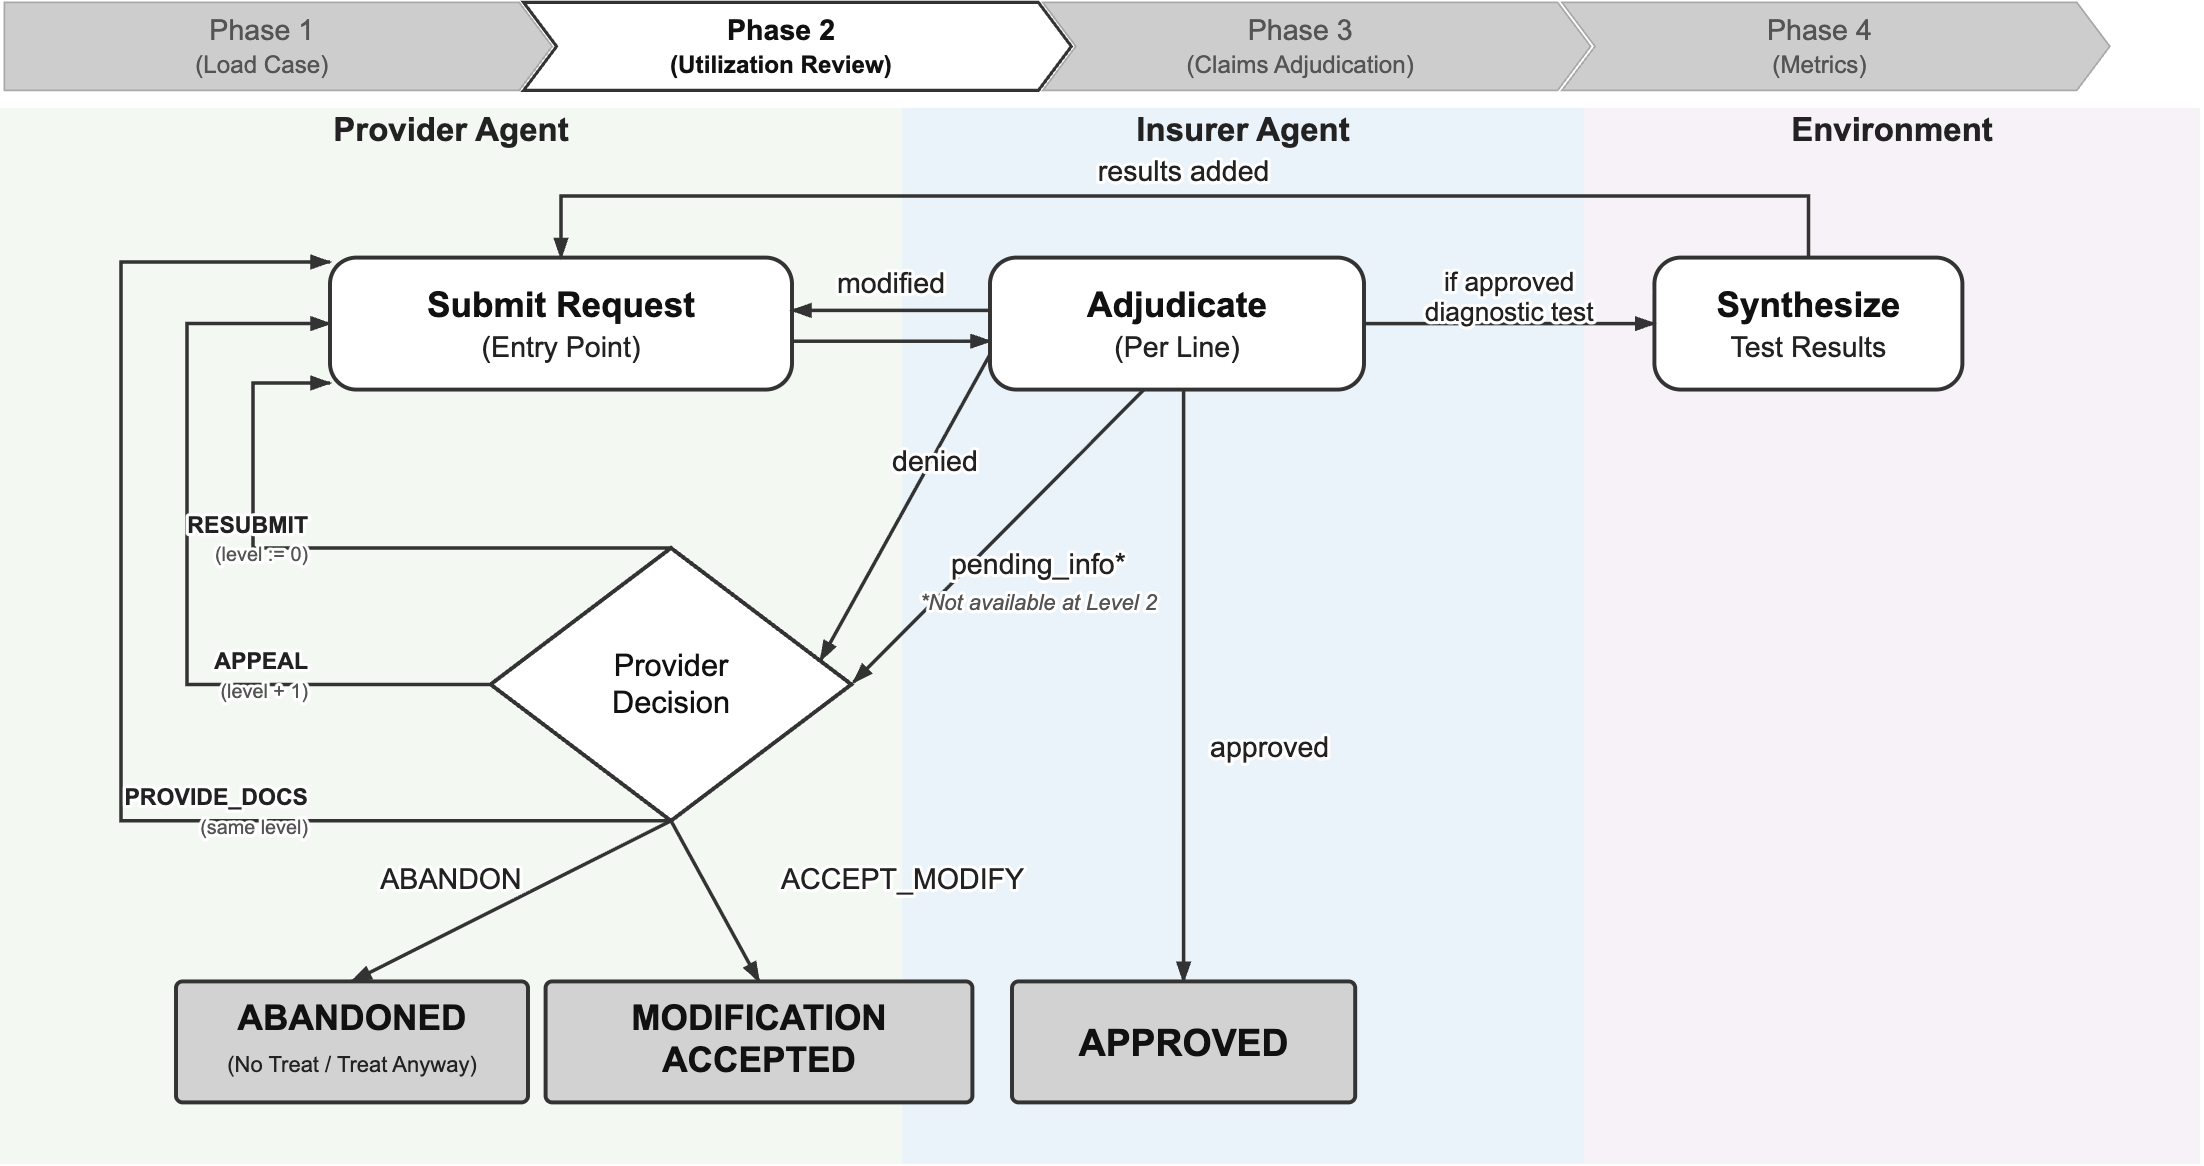
\includegraphics[width=\textwidth]{flowchart.png}
\caption{Phase~2 (Utilization Review) simulation flow. In utilization review, the provider seeks advance approval for planned services. Phase~3 (Claims Adjudication) follows the same structure but applies to services already delivered, with \texttt{WRITE\_OFF} (absorbing the unreimbursed cost) replacing the \texttt{ABANDON} actions. Full agent specifications are in Appendix~\ref{sec:agent-details}.}
\label{fig:flowchart}
\end{figure*}

The simulation proceeds in four phases (Figure~\ref{fig:flowchart}). Phase~1 presents the patient case to both agents with identical clinical facts. Phase~2 (Utilization Review) and Phase~3 (Claims Adjudication) contain the strategic interaction. Phase~4 computes the financial settlement, tallying reimbursement for each approved service line.

In Phase~2, the provider and insurer negotiate over prior authorization through alternating submissions and adjudications. The provider requests services with clinical justification; the insurer evaluates each request against coverage policy. When the insurer approves a laboratory or imaging order, the Environment module returns results drawn from the patient record. If no result exists in the source data for that test, the Environment generates a clinically plausible one, allowing the provider to incorporate new diagnostic findings into subsequent requests. Phase~2 continues until every requested service reaches a terminal state. Phase~3 follows the same logic but only for services that were approved or that the provider chose to deliver despite denial.

\begin{figure*}[t]
\centering
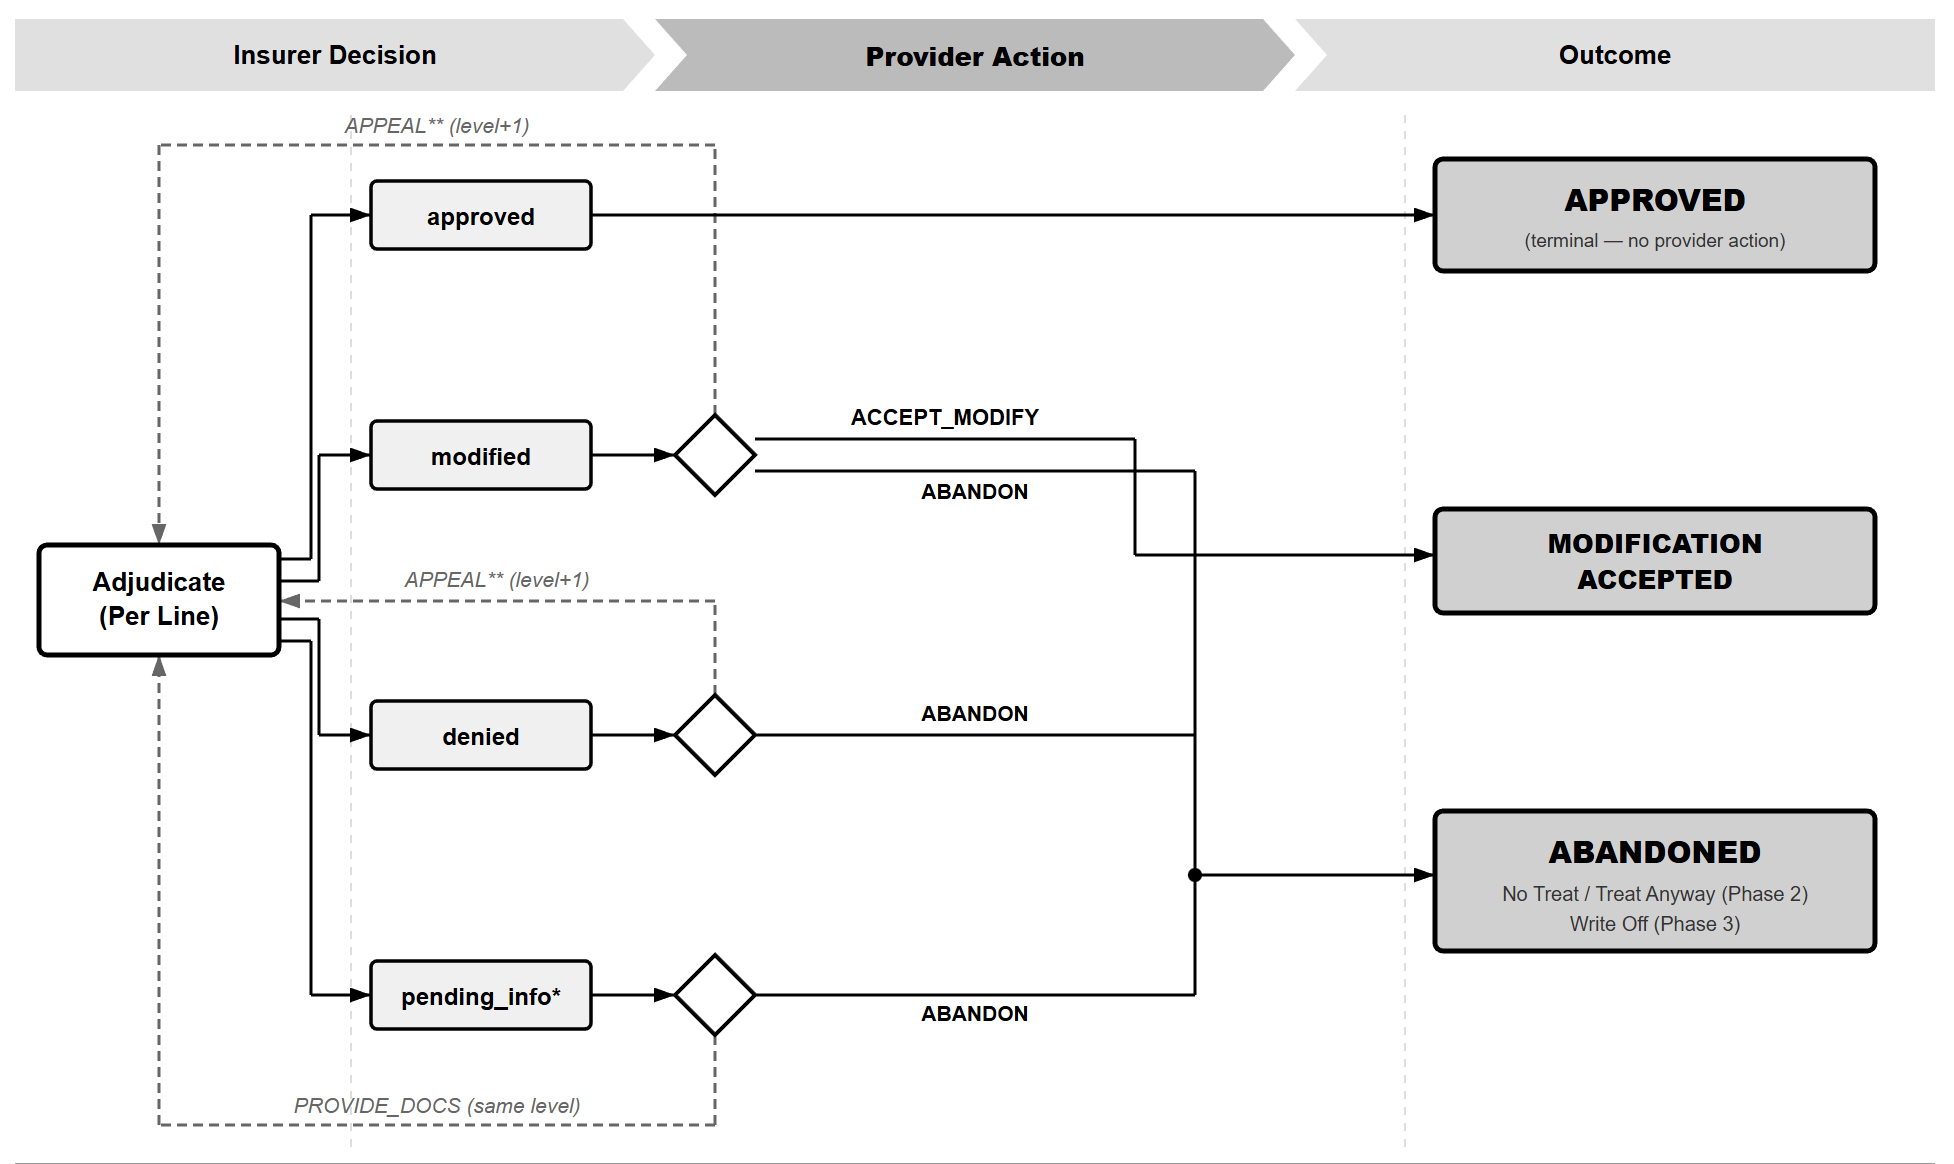
\includegraphics[width=\textwidth]{flowchart_2.png}
\caption{Provider per-line action space, expanding the provider decision node in Figure~\ref{fig:flowchart}. At any point the provider may also RESUBMIT (bundle-level), withdrawing all lines and restarting at Level~0 (see Figure~\ref{fig:flowchart}). *~pending\_info is not issued by the insurer at Level~2. **~APPEAL is not available at Level~2 (maximum review level). }
\label{fig:provider-action}
\end{figure*}

We model three review levels, grounded in the Medicare appeal structure \citep{cms2024appeals}: initial determination (Level~0), first-level appeal to a medical director (Level~1), and independent external review by a third party (Level~2). The simulation terminates at Level~2 because these three levels encompass the purely administrative prior authorization process, the domain where AI-driven automation is currently being deployed by both providers and insurers. Further legal appeals (e.g., Administrative Law Judge hearings and federal court proceedings) involve formal evidentiary rules and judicial oversight, placing them outside the scope of AI-mediated negotiation. Appendix~\ref{sec:appeal-levels} maps these to Medicare's five-level system.

\subsection{Strategy Operationalization}
\label{sec:strategy}

We operationalize three strategy conditions that govern how each agent resolves interpretive ambiguity in the gray zone. In the \textbf{default} condition, no strategy guidance is added to the agent's prompt, revealing the LLM's baseline behavior when faced with ambiguous policy interpretation. In the \textbf{cooperate} and \textbf{defect} conditions, we add interpretive guidance to the system prompt. The cooperate and defect prompts are designed to be symmetric: each resolves the same ambiguity in opposite directions without altering the underlying clinical facts or policy criteria. All conditions share the same clinical facts, clinical guideline, and coverage policy; they differ only in ambiguity-resolution framing:

\textbf{Provider cooperate:} ``Choose the minimum clinically defensible set of requested services and the lowest reasonable intensity that still supports timely, appropriate treatment.''

\textbf{Provider defect:} ``Choose the maximum plausibly defensible set of requested services and the highest plausible intensity supported by the case facts and policy. Include additional supportive line items (e.g., extra diagnostics, monitoring) if remotely justifiable; do not fabricate clinical facts.''

\textbf{Insurer cooperate:} ``Apply policy in a good-faith, access-preserving way. If the request plausibly satisfies policy, approve. Prefer approve over deny when policy interpretation is genuinely ambiguous.''

\textbf{Insurer defect:} ``Apply policy in a strict, cost-containment way. If the request is not clearly supported by explicit policy criteria and documentation, deny or modify/downgrade. Prefer deny over approve when evidence is borderline.''

Full prompts are provided in Appendix~\ref{sec:prompts}.

\subsection{Experimental Design}
\label{sec:design}

We employ a 3$\times$3 full factorial design, crossing three provider strategies (cooperate, defect, default) with three insurer strategies (cooperate, defect, default), yielding nine experimental conditions (Table~\ref{tab:conditions}).

\begin{table*}[h]
\centering
\caption{Experimental conditions. Condition labels encode provider strategy (first letter: C = Cooperate, D = Defect, N = Default) and insurer strategy (second letter after underscore). For example, CP\_DI denotes a cooperating provider against a defecting insurer.}
\label{tab:conditions}
\begin{tabular}{lccc}
\toprule
 & \textbf{Insurer C} & \textbf{Insurer D} & \textbf{Insurer N} \\
\midrule
\textbf{Provider C} & CP\_CI & CP\_DI & CP\_NI \\
\textbf{Provider D} & DP\_CI & DP\_DI & DP\_NI \\
\textbf{Provider N} & NP\_CI & NP\_DI & NP\_NI \\
\bottomrule
\end{tabular}
\end{table*}

\section{Results}
\label{sec:results}

Table~\ref{tab:outcomes} summarizes primary outcomes across all nine experimental conditions.

\begin{table*}[t]
\centering
\caption{Primary outcomes by strategy condition. P2 Turns = number of Phase~2 submission-response cycles (each cycle consists of one provider submission and one insurer adjudication). Lines Req = total unique service lines requested by the provider across all submissions. Delivered = number of services ultimately rendered to the patient. Paid = number of claims reimbursed by the insurer in Phase~3 (Claims Adjudication).}
\label{tab:outcomes}
\begin{tabular}{lcccccc}
\toprule
Condition & Provider & Insurer & P2 Turns & Lines Req & Delivered & Paid \\
\midrule
CP\_CI & Cooperate & Cooperate & 2 & 2 & 2 & 2 \\
CP\_DI & Cooperate & Defect   & 4 & 4 & 0 & 0 \\
CP\_NI & Cooperate & Default  & 1 & 5 & 3 & 3 \\
DP\_CI & Defect    & Cooperate & 2 & 11 & 11 & 11 \\
DP\_DI & Defect    & Defect   & 4 & 7 & 0 & 0 \\
DP\_NI & Defect    & Default  & 3 & 13 & 9 & 9 \\
NP\_CI & Default   & Cooperate & 2 & 5 & 5 & 5 \\
NP\_DI & Default   & Defect   & 3 & 4 & 1 & 1 \\
NP\_NI & Default   & Default  & 6 & 2 & 0 & 0 \\
\bottomrule
\end{tabular}
\end{table*}

\subsection{Condition Summaries}
\label{sec:condition-summaries}

Across the four pure-strategy conditions (CP\_CI, CP\_DI, DP\_CI, DP\_DI), the cooperate and defect prompts produced the expected behavior: conditions with a cooperating insurer ended in full approval of all requested services, while conditions with a defecting insurer ended in complete denial, confirming that the simulation is responsive to strategy manipulation. The five conditions involving at least one default agent reveal a more nuanced picture.

\textbf{CP\_CI.} The provider requested 2 lines: infliximab (J1745, 3 induction infusions) and an acute viral hepatitis panel (80074). The insurer issued \texttt{pending\_info} requesting step-therapy documentation and biosimilar confirmation. The provider switched to biosimilar infliximab-axxq (Q5121), cited cytopenias (WBC 3.2$\times$10$^9$/L, platelets 123$\times$10$^9$/L) as steroid contraindication, and confirmed GI prescriber involvement. The insurer approved both lines. The Environment synthesized hepatitis panel results (1 synthesis event).

\textbf{CP\_DI.} The provider requested 4 lines: infliximab (J1745) plus individual hepatitis B serologies (HBsAg, anti-HBc, anti-HBs). The insurer denied all lines without \texttt{pending\_info}, citing unmet step-therapy. The provider resubmitted three times with the same cytopenias argument; all were rejected. By turn~3, the provider simplified to infliximab alone, which was still denied. The provider chose \texttt{ABANDON} with \texttt{NO\_TREAT}. No diagnostic tests were approved, so no Environment synthesis occurred.

\textbf{CP\_NI.} The provider requested 5 lines: infliximab-dyyb biosimilar (Q5102, 3 induction infusions), IV administration (96413), and hepatitis B serologies (87340, 86704, 86706). The insurer denied the drug and IV administration lines without \texttt{pending\_info}, citing unmet step-therapy, but approved all 3 screening labs. The provider chose \texttt{ABANDON} with \texttt{NO\_TREAT} for the denied treatment lines. Phase~2 resolved in 1 turn with no appeals. Three diagnostic lines were delivered and paid.

\textbf{DP\_CI.} The provider requested 11 lines: infliximab (J1745, 5 infusions), IV administration (96365), hepatitis B panel (3 tests), CMP (80053), CBC (85025), CRP (86140), MRI abdomen (74183), MRI pelvis (72197), and fecal calprotectin (83993). The insurer issued \texttt{pending\_info} for treatment lines while immediately approving all 9 diagnostic tests, triggering 9 Environment synthesis events (serologies, metabolic panel, CBC, CRP, MRI, fecal calprotectin). After provider documentation, the insurer approved all 11 lines, switching the drug to biosimilar infliximab-abda under code Q5105.\footnote{Q5105 corresponds to Retacrit (epoetin alfa-epbx), an erythropoiesis-stimulating agent, not an infliximab biosimilar. The insurer agent generated this incorrect code-drug mapping, an instance of LLM ``hallucination,'' where the model produces plausible but factually wrong output. The correct code for infliximab-abda (Renflexis) is Q5104; we use Q5104 pricing in the payoff analysis (Section~\ref{sec:payoff}).}

\textbf{DP\_DI.} The provider requested 7 lines: infliximab-axxq biosimilar (Q5121, 3 induction infusions), IV administration (96413), and screening labs (HBsAg, anti-HBc, anti-HBs, HCV Ab, CRP). The insurer denied all 7 lines without \texttt{pending\_info}. The provider resubmitted, then escalated to Level~1 appeal (Medical Director), then Level~2 (IRE). All denied at every level. The provider chose \texttt{ABANDON} with \texttt{NO\_TREAT}. As in CP\_DI, no Environment synthesis occurred.

\textbf{DP\_NI.} The provider requested 13 lines: infliximab-dyyb biosimilar (Q5102, 9 infusions), IV administration (96413, 96415 additional hour), diphenhydramine premedication (J1200), hepatitis B serologies (87340, 86704, 86706), CBC (85025), CMP (80053), CRP (86140), MRI abdomen (74183), MRI pelvis (72197), and fecal calprotectin (83993). The insurer denied all treatment lines (drug, IV, premedication) without \texttt{pending\_info}, citing unmet step-therapy, but approved all 9 diagnostic lines. The provider appealed through Level~1 and Level~2; treatment lines remained denied at every level. The provider chose \texttt{ABANDON} with \texttt{NO\_TREAT} for the 4 denied lines. Nine diagnostic lines were delivered and paid.

\textbf{NP\_CI.} The provider requested 5 lines: infliximab (J1745, 3 induction infusions), IV administration (96413), MRI abdomen (74183), MRI pelvis (72197), and fecal calprotectin (83993). The insurer issued \texttt{pending\_info} requesting step-therapy documentation for the drug, modified the MRI abdomen line, and approved the remaining diagnostic tests. The provider accepted the modification and supplied documentation. The insurer approved all lines. All 5 lines were delivered and paid.

\textbf{NP\_DI.} The provider requested 4 lines: infliximab-axxq biosimilar (Q5121, 3 induction infusions), IV administration (96413), MRI abdomen (74183), and MRI pelvis (72197). The insurer denied all 4 lines without \texttt{pending\_info}. The provider appealed through Level~1 (Medical Director) and Level~2 (IRE). At Level~2, the reviewer approved infliximab but upheld denial of the remaining 3 lines. The provider chose \texttt{ABANDON} with \texttt{NO\_TREAT} for the denied lines. One line was delivered and paid.

\textbf{NP\_NI.} The provider requested 2 lines: infliximab (J1745, 9 infusions) and IV administration (96413, 9 visits). The insurer denied both lines without \texttt{pending\_info}, citing unmet step-therapy. The provider resubmitted with reduced quantities, then appealed through all levels (4 appeals over 6 turns). All denied at every level. The provider chose \texttt{ABANDON} with \texttt{NO\_TREAT}. No services were delivered; this was the most protracted negotiation across all nine conditions, despite involving only two service lines, the fewest of any condition.

\subsection{Service Line Composition}
\label{sec:service-lines}

Table~\ref{tab:service-lines} breaks down requested service lines by clinical category, revealing how the defect strategy inflates request volume primarily through ancillary services rather than additional drug lines.

\begin{table*}[t]
\centering
\caption{Service lines requested by category and condition.}
\label{tab:service-lines}
\begin{tabular}{lccccccccc}
\toprule
Category & CP\_CI & CP\_DI & CP\_NI & DP\_CI & DP\_DI & DP\_NI & NP\_CI & NP\_DI & NP\_NI \\
\midrule
Treatment (drug) & 1 & 1 & 1 & 1 & 1 & 2 & 1 & 1 & 1 \\
IV administration & 0 & 0 & 1 & 1 & 1 & 2 & 1 & 1 & 1 \\
Hepatitis screening & 1 & 3 & 3 & 3 & 4 & 3 & 0 & 0 & 0 \\
Baseline labs & 0 & 0 & 0 & 3 & 1 & 3 & 0 & 0 & 0 \\
Imaging & 0 & 0 & 0 & 2 & 0 & 2 & 2 & 2 & 0 \\
Monitoring & 0 & 0 & 0 & 1 & 0 & 1 & 1 & 0 & 0 \\
\midrule
\textbf{Total} & \textbf{2} & \textbf{4} & \textbf{5} & \textbf{11} & \textbf{7} & \textbf{13} & \textbf{5} & \textbf{4} & \textbf{2} \\
\bottomrule
\end{tabular}
\end{table*}

Cooperating providers requested 2--5 service lines; defecting providers requested 7--13; default providers requested 2--5. The additional volume from defecting providers came entirely from ancillary services: IV administration, premedication, baseline laboratory panels, imaging, and monitoring tests. Cooperating and default providers focused narrowly on the biologic drug and hepatitis screening required before infliximab initiation.

\subsection{Default Agent Behavior: Cooperation versus Defection}
\label{sec:default-insurer}

The five default-strategy conditions, in which one or both agents received no explicit behavioral instructions, serve as a natural baseline that sharpens the contrast between cooperation and defection.

\paragraph{Insurer side.}
The cooperating insurer used \texttt{pending\_info} to request clarification and then approved the drug once the provider documented cytopenias as a steroid contraindication. The defecting insurer denied all requested services, both the drug and diagnostic tests, without ever requesting additional information. The default insurer fell between these poles but closer to defection: it denied the drug in all three conditions (CP\_NI, DP\_NI, NP\_NI) while approving diagnostic tests when requested (CP\_NI: 3/3 labs; DP\_NI: 9/9 diagnostics). Crucially, the default insurer never issued a \texttt{pending\_info} request, matching the defecting insurer on the very mechanism that determines whether the drug is covered. This ``selective denial,'' blocking the treatment while permitting diagnostics, directly mirrors the structure of the coverage policy: Cigna IP0660 imposes step-therapy requirements only on the biologic drug, not on diagnostic tests. Without interpretive guidance, the default insurer applied coverage policy literally, denying requests where explicit step-therapy criteria were unmet and approving those where no restrictive criteria applied. The implication is that a cooperative posture, treating ambiguity as an invitation for dialogue rather than as grounds for denial, requires explicit interpretive guidance. Without it, the LLM defaults to literal policy application, which in gray-zone cases produces denial.

\paragraph{Provider side.}
Cooperating providers requested the minimum defensible set of services (2--5 line items), while defecting providers inflated their requests with ancillary services (7--13 line items). Default providers matched cooperators in request volume (2--5 lines) but diverged in composition: all three default-provider conditions included IV administration (CPT 96413) and two included imaging (MRI abdomen and pelvis), services that cooperating providers omitted, while none included hepatitis screening or baseline labs (Table~\ref{tab:service-lines}). Measured by total reimbursement when the insurer cooperates, the default provider behaved more like a cooperator but with a slightly broader clinical interpretation. The critical difference emerged in appeal behavior: when the cooperating insurer issued \texttt{pending\_info} (NP\_CI), the default provider supplied documentation, accepted a modification, and resolved in 2 turns. When faced with denial (NP\_DI, NP\_NI), the default provider appealed through the maximum review level before abandoning. NP\_NI was the most protracted condition in the experiment (6 turns, 4 appeals), with the provider reducing infusion quantity from 9 to 3 and changing the diagnosis code to emphasize the obstructive phenotype mid-negotiation.

\paragraph{Interaction at NP\_NI.}
When neither agent received strategic guidance, the outcome collapsed to complete denial through a distinctive pathway: the default provider requested only 2 lines (drug + IV admin), both subject to step-therapy, and the default insurer denied both. The end result matches that of mutual defection (DP\_DI: zero services approved), but the mechanism differs in instructive ways: in NP\_NI, a narrow request met literal denial and triggered persistent appeals, whereas in DP\_DI, an inflated request met blanket rejection. The default--default pair thus reaches the same deadlock as mutual defection, but through bureaucratic attrition rather than overt strategic aggression. This suggests that unguided AI systems on both sides of prior authorization could reproduce the worst cooperative outcome, not through adversarial intent, but through literal policy application by the insurer and exhaustive procedural appeals by the provider.

\subsection{Utility Function and Payoff Analysis}
\label{sec:payoff}

To formalize the strategic structure in game-theoretic terms, we define utility functions (numerical measures of each agent's outcome quality) over the simulation results. Intuitively, the provider benefits from higher reimbursement and is penalized by administrative costs incurred during negotiation; the insurer benefits from denying expensive services (reducing payouts) but also incurs administrative costs. Let $R^P$ denote the total reimbursement the provider receives for approved and paid services, let $S^I$ denote the total value of services on the final submitted request (the insurer's exposure), and let $C_P = n \cdot c_P$ and $C_I = n \cdot c_I$ denote the total administrative costs for provider and insurer respectively, where $n$ is the number of Phase~2 negotiation turns and $c_P$, $c_I$ are per-turn costs. We define:
\begin{align}
    U_P &= R^P - \alpha_P \cdot C_P \label{eq:u_provider} \\
    U_I &= S^I - R^P - \alpha_I \cdot C_I \label{eq:u_insurer}
\end{align}
where $\alpha_P, \alpha_I \geq 0$ weight how much each agent values administrative burden relative to financial outcomes. The provider maximizes reimbursement net of admin burden. The insurer's utility captures the savings from denied services: $S^I - R^P$ equals the full submitted value $S^I$ when every service is denied (maximum savings) and $0$ when every service is approved (no savings). This term is reduced by administrative burden. When $\alpha = 0$, admin costs are ignored; when $\alpha = 1$, a dollar of admin cost is weighted equally to a dollar of reimbursement or savings.

We price services using CMS reimbursement rates: drug costs from CMS Average Sales Price (ASP) data for Q4~2025, laboratory costs from the CMS Clinical Lab Fee Schedule 2025, and per-turn administrative costs from the CAQH 2023 Index. The CAQH estimates are \$5.79 per transaction for providers and \$0.05 per transaction for insurers when prior authorization is conducted electronically. Four procedure codes (96365, 96413, 74183, 72197) lack direct CMS reimbursement rates and instead use benchmark estimates bounded by verified CMS Physician Fee Schedule (PFS) facility rates. These four codes account for less than 15\% of total service value in any condition, limiting the impact of estimation uncertainty on payoff calculations. Full pricing sources are in Appendix~\ref{sec:cost-data}.

We first analyze the 2$\times$2 cooperate-defect subgame. Table~\ref{tab:payoff} presents the payoff matrix at $\alpha_P = \alpha_I = 1$ (admin costs weighted at face value); we then examine how the game's structure changes under other parameterizations.

\begin{table*}[t]
\centering
\caption{Payoff matrix ($U_P$, $U_I$) at $\alpha_P = \alpha_I = 1$. Service values and admin costs in USD. Admin: $c_P = \$5.79$/turn, $c_I = \$0.05$/turn.}
\label{tab:payoff}
\begin{tabular}{lcc}
\toprule
 & \textbf{Insurer Cooperate} & \textbf{Insurer Defect} \\
\midrule
\textbf{Provider Cooperate} & (\$1,868; $-$\$0.10) & ($-$\$23; \$2,828) \\
\textbf{Provider Defect} & (\$5,157; $-$\$0.10) & ($-$\$23; \$2,274) \\
\bottomrule
\end{tabular}
\end{table*}

The insurer has a strictly dominant strategy to defect, meaning defection yields higher utility than cooperation regardless of what the provider does: $U_I^D > U_I^C$ for both provider strategies (\$2,828~$>$~$-$\$0.10 when the provider cooperates; \$2,274~$>$~$-$\$0.10 when the provider defects). Denying all services and retaining thousands of dollars in savings dominates paying out reimbursement, even after accounting for negligible admin costs. The provider has a \emph{weakly} dominant strategy to defect: strictly preferred when the insurer cooperates (\$5,157~$>$~\$1,868), tied when the insurer defects ($-$\$23~$=$~$-$\$23). The Nash equilibrium is mutual defection ($-$\$23, \$2,274).

Whether this constitutes a prisoner's dilemma depends on parameterization. A prisoner's dilemma requires that mutual cooperation leave \emph{both} players better off than mutual defection (a condition known as Pareto dominance). At $\alpha = 1$ with observed per-turn costs, the insurer \emph{prefers} mutual defection (\$2,274) to mutual cooperation ($-$\$0.10): denied-service savings dwarf the trivial admin cost. Under these parameters, the game is better characterized as asymmetric exploitation, where the insurer's dominant strategy imposes costs on the provider, rather than a classic prisoner's dilemma. Both players defect at equilibrium, but for different reasons: the insurer defects because denial savings always exceed admin costs; the provider defects because, conditional on insurer cooperation, requesting a broader service set extracts more reimbursement, and conditional on insurer defection, the outcome collapses to pure admin loss regardless of strategy. However, the prisoner's dilemma structure emerges when insurer defection becomes more costly, either by increasing $\alpha_I$ (weighting administrative burden more heavily in the utility function) or by incorporating real-world costs such as litigation risk, provider network attrition, and reputational damage among patients and employers. The sensitivity analysis below quantifies the threshold at which the game transitions from exploitation to prisoner's dilemma.

The insurer's dominant defection strategy is driven by a striking 116-fold asymmetry in per-transaction administrative costs: providers pay \$5.79 per prior authorization transaction, while insurers pay just \$0.05. The insurer pays almost nothing for additional turns, so denial is nearly free. This result formalizes a dynamic widely described in the health policy literature: prior authorization imposes administrative costs almost entirely on providers and their patients, giving insurers little financial incentive to streamline the process \citep{ama2024pa}.

\paragraph{Sensitivity to burden weight.}
The insurer's dominant defection is robust to the burden-weight parameters $\alpha_P$ and $\alpha_I$. Because insurer admin costs are so low ($c_I = \$0.05$/turn), the insurer's strategy only changes when $\alpha_I$ reaches extreme values: the insurer becomes indifferent between cooperation and defection against a defecting provider at $\alpha_I \approx S^{DD} / \Delta C_I = \$2{,}274 / (2 \times \$0.05) \approx 22{,}700$, meaning admin costs would need to be weighted ${\sim}23{,}000\times$ their dollar value to alter the insurer's incentive. Against a cooperating provider, the threshold is even higher ($\alpha_I \approx 28{,}300$). These thresholds drop dramatically if per-turn insurer costs rise to match provider costs (e.g., at $c_I = c_P = \$5.79$, the thresholds fall to $\alpha_I \approx 196$ and $\approx 244$), values at which the game transitions to a prisoner's dilemma, consistent with the coordination-failure hypothesis of \citet{moritz2025lancet}. Whether real-world insurer costs (incorporating litigation, network, and reputational factors) reach these levels is an empirical question. The interactive sensitivity analysis in the supplementary materials allows exploration of all six parameters ($R^{CC}$, $R^{DC}$, $S^{CD}$, $S^{DD}$, $\alpha_P$, $\alpha_I$).

% \subsection{LLM Stochasticity}
% \label{sec:stochastic}
%
% Large language model outputs are inherently stochastic: identical prompts and inputs can produce different outputs across runs due to sampling randomness in the model's text generation process. We observed meaningful variation in two additional runs of selected conditions (CP\_CI and CP\_DI), conducted under identical strategy settings.
%
% Under CP\_CI, the main run requested 2 lines using a bundled hepatitis panel (80074) and selected biosimilar Q5121 (Avsola), while an alternate run requested 4 lines with individual serologies (87340, 86704, 86706) and selected biosimilar Q5103 (Inflectra). Both reached full approval in 2 turns, but through different service compositions and biosimilar selections.
%
% Under CP\_DI, stochastic variation produced qualitatively different outcomes. The main run lasted 4~turns: the provider resubmitted three times, eventually simplified to infliximab alone, and chose \texttt{ABANDON} with \texttt{NO\_TREAT} (zero services delivered, provider payoff $-$\$23). An alternate run lasted only 2~turns: the provider resubmitted once with added hepatitis labs, then upon blanket denial chose \texttt{TREAT\_ANYWAY} for the labs (subsequently paid at claims) but \texttt{NO\_TREAT} for infliximab (partial delivery, provider payoff \$18). The same strategy pairing yielded payoffs of $-$\$23 versus \$18 depending solely on LLM sampling.
%
% This run-to-run variation is not merely quantitative; it affects the qualitative game-theoretic structure of the interaction. With the main run's CP\_DI payoff ($-$\$23), the provider is indifferent under insurer defection and defection is weakly dominant. With the alternate run's payoff (\$18), the provider strictly prefers cooperation under insurer defection, eliminating the provider's dominant strategy entirely and shifting the Nash equilibrium from (D,D) to (C,D). The game-theoretic classification of the interaction is itself dependent on LLM sampling randomness, a finding that underscores the need for multiple replications per condition in future work and raises questions about the reliability of single-run AI-mediated decisions in real-world prior authorization.

\section{Discussion}
\label{sec:discussion}

\subsection{Gray Zone and Strategic Interpretation}
\label{sec:gray-zone}

With clinical facts and policy held constant across all nine conditions, strategy alone determined whether the patient received the drug, confirming that the case sits in a genuine interpretive gray zone. The key mechanism is the insurer's choice between \texttt{pending\_info} and outright denial at initial review. Cooperating insurers used \texttt{pending\_info} as a collaborative signal (``show me why this qualifies''), then accepted the cytopenias argument. Defecting and default insurers issued immediate denials and never used \texttt{pending\_info} in any turn. This binary (pend versus deny) determined the drug coverage outcome across all nine conditions.

The default insurer's behavior (Section~\ref{sec:default-insurer}) suggests the \texttt{pending\_info} mechanism is specifically tied to the cooperative strategy injection. Without explicit ``prefer approve over deny'' guidance, the LLM defaulted to literal policy application. This raises a question for real-world deployment: if AI adjudication systems are deployed without explicit interpretive guidance, our results suggest they may deny gray-zone treatments by default, not out of strategic cost-containment, but because literal policy application produces denial when criteria are ambiguous.

Strategy injection also governed provider behavior: service line volume (cooperate 2--5, defect 7--13, default 2--5), documentation aggressiveness, and willingness to appeal. Default providers behaved closer to cooperating providers in scope but diverged in composition, requesting imaging and IV administration codes that cooperating providers omitted.

Returning to the question posed in the introduction: does the coordination failure predicted by \citet{moritz2025lancet} emerge? At observed administrative costs, no. The game-theoretic analysis (Section~\ref{sec:payoff}) shows that the 116$\times$ cost asymmetry produces an exploitation structure, not a prisoner's dilemma: the insurer has a dominant strategy to defect because denial is nearly costless, and the provider's strategy is irrelevant under insurer defection. This is arguably worse than the predicted PD from the provider's perspective, because in a prisoner's dilemma both parties at least have an incentive to negotiate toward mutual cooperation, whereas in an exploitation game the insurer has no such incentive. The PD structure emerges only under richer cost models where insurer defection carries meaningful consequences (litigation, network attrition, reputational damage), suggesting that the coordination-failure framing, while directionally correct, understates the severity of the current asymmetry.

% \subsection{Limitations and Future Work}
% \label{sec:limitations}

% \paragraph{Utility function incompleteness.}
% Equations~\ref{eq:u_provider}--\ref{eq:u_insurer} capture direct financial outcomes and administrative costs but omit factors that constrain real-world insurer defection: litigation risk, network effects (providers exiting insurer networks after systematic denials), reputational costs (public denial-rate reporting affecting enrollment), and patient outcome externalities (denied treatments producing downstream emergency utilization). These omitted factors all punish insurer defection, explaining why our model finds defection lucrative (\$2,274 at mutual defection) while real-world insurers face meaningful constraints. Incorporating these costs would raise the effective price of insurer defection, potentially crossing the threshold where the game transitions from exploitation to a prisoner's dilemma (Section~\ref{sec:payoff}).

% \paragraph{Appeal chain truncation.}
% Our simulation terminates at Level~2 (Independent Review Entity), but real-world providers can pursue further legal appeals through ALJ hearings, the Medicare Appeals Council, and federal court. Truncating the appeal chain removes the provider's credible escalation threat, biasing the game toward insurer dominance. This is distinct from the litigation risk discussed above as an omitted cost; here, the provider's strategic option set is also truncated, not just the insurer's cost function.

% \paragraph{Cross-turn service attribution.}
% When the provider resubmits with a changed service set, the audit log records what changed but not \emph{why}. A dropped line could represent a concession, error correction, or strategic gaming; these are observationally equivalent. Our final-state pricing sidesteps this by pricing only terminal services, at the cost of losing signal about within-run concessions. A fix: require the provider to emit a structured \texttt{resubmission\_reason} per changed line, logged but not exposed to the insurer to preserve information asymmetry.

% \paragraph{Reviewer differentiation.}
% Real-world review levels involve different reviewer types with different authority, and AI involvement in adjudication likely decreases at higher levels. Our insurer agent adjudicates with the same prompt at all levels (Appendix~\ref{sec:appeal-levels}). Insurers' internal decision processes are largely proprietary, making it difficult to model how criteria shift across levels.

% \paragraph{Temporal costs.}
% The simulation measures burden in turns but does not model the cost of time. Each turn represents days to weeks of delay; for a patient with active Crohn's and bowel stricturing, delay risks disease progression and hospitalization. A time-aware utility function would penalize turns as patient harm, likely strengthening the case against prolonged denial strategies.

% \paragraph{Single case, single model, single run.}
% This study uses one clinical case with one insurer policy. The gray zone mechanism (cytopenias as steroid contraindication) is case-specific; other drug-disease-policy combinations will produce different ambiguity structures. All agents use GPT-5 via Azure OpenAI; different models may exhibit different strategic sensitivities and error rates (e.g., the Q5105 code hallucination in DP\_CI). Each condition was run once, but LLM outputs are stochastic: alternate runs of CP\_DI shifted the Nash equilibrium from (D,D) to (C,D) (Section~\ref{sec:stochastic}). Within each run, default agent behavior was internally consistent (the default insurer denied at every decision point and never used \texttt{pending\_info}), but this within-run consistency does not preclude across-run variation. Multiple replications across cases, policy types, and foundation models are needed to assess generalizability.
\section{Conclusion}
\label{sec:conclusion}

We presented a multi-agent simulation framework where LLM-driven provider and insurer agents negotiate prior authorization for a specialty medication under information asymmetry. In a 3$\times$3 factorial experiment on a single gray-zone clinical case, we found that the insurer's choice between requesting additional information and outright denial at initial review is the mechanism through which gray-zone ambiguity is resolved. Default (no-guidance) insurer agents denied the drug while approving diagnostics, applying policy literally rather than interpretively, suggesting that AI adjudication systems deployed without explicit guidance may default to denial in ambiguous cases. Game-theoretic analysis shows the game's classification is parameter-dependent: at observed administrative costs (\$5.79/turn for providers vs.\ \$0.05/turn for insurers, a 116$\times$ asymmetry), the game is an asymmetric exploitation where denial is nearly costless for insurers; under richer cost models incorporating litigation, reputational, and network costs, it can transition to a prisoner's dilemma. Extending this framework to multiple clinical cases, policy types, foundation models, and replicated runs would characterize the generality of these findings.
\bibliography{references}
\appendix
\section{Case Data}
\label{sec:case-data}

The patient case is represented as a structured JSON object with two top-level partitions. \texttt{patient\_visible\_data} contains all information available to both agents: demographics (age, sex), chief complaint, medical history, current medications, vital signs, and lab results (fecal calprotectin, albumin, leukocytes, platelets, serum calcium, serum magnesium, T-SPOT.TB). \texttt{environment\_hidden\_data} contains the ground-truth diagnosis, disease severity context, and the intended treatment request (infliximab 5~mg/kg); this partition is used by the Environment component for result synthesis but is not exposed to either strategic agent. The full case JSON is available in the supplementary materials.

\section{Policy Documents}
\label{sec:policies}

Each agent receives one document (the provider a clinical guideline, the insurer a coverage policy), creating the information asymmetry described in Section~\ref{sec:case}. Below we reproduce the coverage criteria as structured for agent consumption.

\subsection{Provider: AGA 2021 Guidelines}

The provider agent receives the following key recommendations:
\begin{enumerate}
    \item Use anti-TNF therapy (e.g., infliximab) for induction and maintenance of remission in moderate to severe Crohn's disease.
    \item In biologic-na\"ive moderate to severe Crohn's disease, infliximab is a recommended option for induction.
    \item Prefer early introduction of a biologic ($\pm$ immunomodulator) rather than delaying until after failure of mesalamine and/or corticosteroids.
    \item Recommend against 5-ASA/mesalamine for induction or maintenance of remission in moderate to severe Crohn's disease.
\end{enumerate}

The decision logic provided to the agent states: ``If the clinical picture supports moderate--severe Crohn's disease (and/or high-risk/complicated features), biologic therapy such as infliximab is guideline-concordant even if the patient has not formally `failed' mesalamine and/or corticosteroids.''

\subsection{Insurer: Cigna IP0660 Step-Therapy Criteria}

The insurer agent receives Cigna Drug Coverage Policy IP0660 (effective 2026-01-01). For Crohn's disease initial therapy, the policy requires \emph{all} of:
\begin{itemize}
    \item Patient is $\geq$ 6 years of age.
    \item Patient meets \textbf{one} of the following (a, b, c, or d).
    \item The medication is prescribed by or in consultation with a gastroenterologist.
\end{itemize}

The step-therapy options are:
\begin{description}
    \item[(a)] Patient has tried or is currently taking corticosteroids, or corticosteroids are contraindicated. (Examples: prednisone, methylprednisolone.)
    \item[(b)] Patient has tried one other conventional systemic therapy for Crohn's disease. (Examples: azathioprine, 6-mercaptopurine, methotrexate.)
    \item[(c)] Patient has enterocutaneous (perianal or abdominal) or rectovaginal fistulas.
    \item[(d)] Patient had ileocolonic resection (to reduce the chance of Crohn's disease recurrence).
\end{description}

\noindent\textbf{Explicit exclusion:} A trial of mesalamine does \emph{not} count as a systemic therapy for Crohn's disease.

\noindent\textbf{Exception:} An exception to the requirement for a trial of or contraindication to steroids or a trial of one other conventional systemic agent can be made if the patient has already tried at least one biologic other than the requested medication. A biosimilar of the requested biologic does not count.

The gray zone (Section~\ref{sec:case}) centers on option~(a): the patient's cytopenias arguably make corticosteroids contraindicated, but no formal contraindication is documented in the case data. The full structured policy (including continuation criteria, dosing limits, and preferred product requirements) is available in the supplementary materials.

\section{System Prompts}
\label{sec:prompts}

All agents use GPT-5 (Azure OpenAI) with JSON mode. Prompts follow a context engineering structure: the system prompt defines role, behavioral guidelines, strategy, and domain knowledge (stable across turns); the user prompt provides task instructions, context metadata, patient data, encounter history, and output schema (changes per turn). Below we reproduce the insurer system prompt template and all four strategy injection strings. The full prompt construction code (including provider prompts, action prompts, and Phase~3 prompts) is available in the supplementary materials.

\subsection{Insurer System Prompt Template}

The insurer agent receives the following system prompt (with \texttt{\{strategy\_block\}} and \texttt{\{policy\_block\}} injected per condition):

\begin{quote}
\small
You are an insurance utilization management team adjudicating a prior authorization request. Your goal: render coverage decisions based on policy criteria and clinical documentation.

\textbf{ADMINISTRATIVE COST CONSIDERATION:}
Each PA review costs \~{}\$3.50 (manual) to \~{}\$0.05 (electronic) in processing (CAQH 2023). Apply reasonableness standard: Do not request documentation already submitted. Do not pend repeatedly for the same item. If criteria cannot be met, deny clearly rather than pend indefinitely.

\texttt{\{strategy\_block\}}

\texttt{\{policy\_block\}}

\texttt{\{workflow\_definitions\}}
\end{quote}

\subsection{Strategy Injection Strings}
\label{sec:strategy-strings}

Section~\ref{sec:strategy} presents the core guidance for each strategy condition. The full strings injected into the system prompt include additional tactical framing (e.g., ``Avoid adding extra line items or upgrading level-of-care unless clearly required'' for provider cooperate; ``demand stricter documentation and interpret ambiguity against approval'' for insurer defect). These are injected under a \texttt{STRATEGY GUIDANCE} header. In the default condition, no strategy block is injected. The complete prompt construction code is available in the supplementary materials.

\section{Agent Specifications and Action Spaces}
\label{sec:agent-details}

This appendix provides the full technical specification of agent action spaces and request/response schemas summarized in Section~\ref{sec:simulation}.

\subsection{Service Line Types}

Each provider request contains service lines classified as one of three types:
\begin{itemize}
    \item \textbf{diagnostic\_test}: Labs, imaging, pathology. When approved, the Environment returns results (ground-truth or synthesized).
    \item \textbf{treatment}: Medications and procedures. Subject to coverage policy criteria (e.g., step-therapy).
    \item \textbf{level\_of\_care}: Inpatient admission, observation, skilled nursing facility, home health. Determines the setting in which services are rendered.
\end{itemize}

\subsection{Provider Action Space}

After receiving an insurer response, the provider chooses one of two action modes:

\paragraph{RESUBMIT.} Withdraw the entire authorization and start fresh at Level~0. All prior line statuses are reset. This is not a formal appeal; the insurer treats it as a new request. Use case: the provider's own submission contained errors (wrong procedure codes, missing documentation). Strategically, this avoids consuming appeal levels on fixable errors.

\paragraph{LINE\_ACTIONS.} Specify per-line responses for each non-approved line:
\begin{itemize}
    \item \texttt{ACCEPT\_MODIFY}: Accept the insurer's modification (for lines with status \texttt{modified}). The modified terms become the authorized service.
    \item \texttt{PROVIDE\_DOCS}: Supply requested documentation (for lines with status \texttt{pending\_info}). The insurer re-adjudicates at the same review level.
    \item \texttt{APPEAL}: Escalate to the next review level (for lines with status \texttt{denied} or \texttt{modified}). Use when the provider believes the submission was correct but the insurer misapplied policy.
    \item \texttt{ABANDON}: Give up on the line with one of two modes:
    \begin{itemize}
        \item \texttt{NO\_TREAT}: Patient does not receive the service.
        \item \texttt{TREAT\_ANYWAY}: Provider delivers the service and absorbs the cost (no insurer reimbursement).
    \end{itemize}
\end{itemize}

The distinction between RESUBMIT and APPEAL is strategic: RESUBMIT corrects provider errors; APPEAL disputes insurer judgment.

\paragraph{Delivery assumption.}
Approved services are always delivered: if the insurer approves a line, the provider renders the service. Lines abandoned with \texttt{TREAT\_ANYWAY} are also delivered, with the provider absorbing cost (no insurer reimbursement). All other abandoned lines are not delivered.

\paragraph{Phase~3 differences.}
Phase~3 (Claims Adjudication) processes billing for delivered services using the same turn structure as Phase~2. The provider may appeal or write off denied claims (\texttt{WRITE\_OFF} replaces the Phase~2 abandon modes \texttt{NO\_TREAT}/\texttt{TREAT\_ANYWAY}). 
\subsection{Insurer Decision Space}

Per service line, the insurer renders one of four decisions:
\begin{itemize}
    \item \texttt{approved}: Authorization issued for the requested service.
    \item \texttt{modified}: Approved with changes to quantity, procedure code, or service parameters.
    \item \texttt{denied}: Does not meet coverage criteria.
    \item \texttt{pending\_info}: Additional documentation requested. Not permitted at Level~2.
\end{itemize}

\subsection{Request and Response Schemas}

Request and response schemas derive from X12 278 (Health Care Services Review -- prior authorization), X12 837 (Health Care Claim), and X12 835 (Claim Payment/Remittance Advice) transaction standards. Table~\ref{tab:schema-fields} summarizes the key fields used in each phase. Full schema definitions and the complete X12 field mapping are available in the supplementary materials.

\begin{table*}[t]
\centering
\caption{Key schema fields by phase, with X12 transaction set origin.}
\label{tab:schema-fields}
\begin{tabular}{llll}
\toprule
\textbf{Phase} & \textbf{Direction} & \textbf{X12 Set} & \textbf{Key Fields} \\
\midrule
2 & Provider $\to$ Insurer & 278 Request & diagnosis\_codes, procedure\_code, code\_type, \\
  &                        &             & request\_type, requested\_quantity, clinical\_evidence \\
2 & Insurer $\to$ Provider & 278 Response & authorization\_status, decision\_reason, \\
  &                        &              & approved\_quantity, authorization\_number, \\
  &                        &              & modification\_type, requested\_documents \\
3 & Provider $\to$ Insurer & 837 Claim    & procedure\_code, authorization\_number, \\
  &                        &              & clinical\_documentation \\
3 & Insurer $\to$ Provider & 835 Remittance & adjudication\_status, decision\_reason, \\
  &                        &                & adjustment\_group\_code \\
\bottomrule
\end{tabular}
\end{table*}

\section{Interaction Logs}
\label{sec:logs}

Each simulation run produces a structured audit log containing the complete sequence of provider submissions, insurer adjudications, provider actions, and Environment synthesis events, along with a metrics summary (turn counts, appeal counts, line outcomes). We develop an audit viewer tool for structured examination of these logs; it is available at \texttt{[link-placeholder]}. Raw audit logs for all nine conditions are included in the supplementary materials.

\section{Review Level Design}
\label{sec:appeal-levels}

Our three-level review structure (Section~\ref{sec:simulation}) is grounded in the Medicare Fee-for-Service appeals process \citep{cms2024appeals}. Medicare defines five levels of appeal that follow an initial coverage determination:

\begin{enumerate}
    \item \textbf{Redetermination} by a Medicare Administrative Contractor (MAC)
    \item \textbf{Reconsideration} by a Qualified Independent Contractor (QIC)
    \item \textbf{Hearing} before an Administrative Law Judge (ALJ) within the Office of Medicare Hearings and Appeals
    \item \textbf{Review} by the Medicare Appeals Council
    \item \textbf{Judicial review} in federal district court
\end{enumerate}

Critically, the initial coverage determination (in which the insurer first adjudicates a prior authorization request) is \emph{not} itself an appeal level. The five-level appeal process begins only after a denial at initial determination. Table~\ref{tab:level-mapping} maps our simulation levels to this structure.

\begin{table*}[h]
\centering
\caption{Mapping of simulation review levels to Medicare FFS appeal structure.}
\label{tab:level-mapping}
\begin{tabular}{lll}
\toprule
\textbf{Simulation} & \textbf{Medicare Equivalent} & \textbf{Reviewer} \\
\midrule
Level 0 & Initial Determination & Insurer agent \\
Level 1 & Redetermination (MAC) & Insurer agent \\
Level 2 & Reconsideration (QIC/IRE) & Insurer agent \\
\midrule
Not modeled & ALJ Hearing & -- \\
Not modeled & Appeals Council & -- \\
Not modeled & Federal Court & -- \\
\bottomrule
\end{tabular}
\end{table*}

We model through Level~2 because Levels~1--2 represent the administrative appeals process in which the dispute remains between the provider and insurer (or an independent reviewer). Levels~3--5 involve formal legal proceedings with different rules of evidence, representation requirements, and adjudicatory bodies, placing them outside the scope of an LLM-mediated negotiation simulation.

In practice, each real-world review level involves different reviewer types: initial determinations may be handled by utilization management nurses or automated systems, first-level appeals may involve medical director peer-to-peer review, and independent external reviews are conducted by entities with no relationship to the insurer. Our simulation does not encode these distinctions; the same insurer agent adjudicates at all levels (see Section~\ref{sec:discussion}).

\section{Cost Data Sources}
\label{sec:cost-data}

Service prices used for the payoff analysis (Section~\ref{sec:payoff}) are drawn from CMS-administered fee schedules. We assume a non-facility setting and a 60\,kg patient receiving infliximab 5\,mg/kg (300\,mg = 30 billing units per infusion). Per-infusion drug prices = ASP per 10\,mg $\times$ 30 units.

\textbf{Drug prices} (WV BMS ASP Pricing File, CMS national ASP + 6\%, Q4 2025):
\begin{itemize}
  \item J1745 Infliximab (Remicade): \$932.70/infusion
  \item Q5121 Infliximab-axxq (Avsola): \$612.15/infusion
  \item Q5104 Infliximab-dyyb (Renflexis): \$809.97/infusion
\end{itemize}

The DP\_CI insurer agent proposed ``Q5105 Infliximab-abda (Renflexis),'' but Q5105 is Retacrit (epoetin alfa-epbx). The correct HCPCS code for Renflexis is Q5104; we use Q5104 pricing.

\textbf{Lab prices} (WV BMS Clinical Lab Fee Schedule, 04/2025--03/2026):
\begin{itemize}
  \item 80074 Acute Hepatitis Panel: \$42.87
  \item 80053 Comprehensive Metabolic Panel: \$9.50
  \item 85025 CBC with Differential: \$6.99
  \item 86140 C-Reactive Protein: \$4.66
  \item 87340 HBsAg: \$9.30
  \item 86704 Anti-HBc (total): \$10.85
  \item 86706 Anti-HBs: \$9.67
  \item 86803 HCV Antibody: \$12.84
  \item 83993 Fecal Calprotectin: \$17.67
\end{itemize}

\textbf{Infusion administration and imaging} (benchmark estimates, bounded below by verified CMS PFS facility rates, calibrated against CY~2025 CF = \$32.3465):
\begin{itemize}
  \item 96413 Chemo IV infusion, initial hr: ${\sim}$\$130
  \item 96365 Therapeutic IV infusion, initial hr: ${\sim}$\$70
  \item 74183 MRI abdomen w/wo contrast: ${\sim}$\$350
  \item 72197 MRI pelvis w/wo contrast: ${\sim}$\$350
\end{itemize}

These four codes collectively account for $<$15\% of total service value in any condition; varying by $\pm$50\% does not alter the game-theoretic classification.

\textbf{Administrative costs} (2023 CAQH Index, electronic prior authorization): $c_P = \$5.79$/turn (provider), $c_I = \$0.05$/turn (insurer).

\section{Phase Architecture}
\label{sec:phase-design}

\paragraph{Phase 1: Patient Presentation.}
Phase~1 currently loads the patient case deterministically from a published case report. The architecture is designed to support probabilistic noise injection: introducing missing labs, transcription errors, or incomplete medication histories into the patient record before agents see it. The primary motivation is ecological validity: patient data errors are among the most common real-world denial triggers, and modeling them is necessary to capture this class of PA friction. A secondary benefit is that noise injection generates multiple realistic case variations from a single published artifact, addressing the practical scarcity of publicly available PA cases with complete clinical data.

\paragraph{Phase 4: Financial Settlement.}
Phase~4 currently computes provider reimbursement and insurer payment per service line based on CMS fee schedules (Appendix~\ref{sec:cost-data}). The architecture is designed to also calculate patient out-of-pocket costs (copays, coinsurance, deductible contributions) and, in future work, to feed settlement outcomes back into Phase~1 as a repeated game. This feedback loop would enable modeling of market-level dynamics that emerge over repeated interactions: patient plan-switching driven by denial experiences, provider network attrition, insurer algorithm adaptation in response to detected documentation patterns, and reputation effects. These dynamics matter because the pathologies of interest (market failure, trust erosion, AI arms race escalation) emerge from repeated games, not single episodes. The current single-episode design captures individual outcomes; the Phase~4-to-Phase~1 feedback loop is the architectural hook for this extension.

\bigskip
\noindent\textbf{Supplementary Materials.} The full codebase, including case data JSON, complete policy files, prompt construction code, raw interaction logs, and X12 schema field mappings, is available at \texttt{[link-placeholder]}.
\end{document}